\documentclass[a4paper,onesided,12pt]{report} 

\usepackage{EMU_ThesisPHD2}
\usepackage{amsmath}
\usepackage{amssymb}
\usepackage{graphicx}
\usepackage{esint}
\usepackage{pslatex}
\usepackage{graphics}
\usepackage{cite}
\usepackage{pgfplots}
\pgfplotsset{width=10cm,compat=1.9}
\usepgfplotslibrary{external}

\tikzexternalize
\setcounter{MaxMatrixCols}{10}

\pagestyle{plain}

\degree{ Ph.D. in Physics }
\subyear{2016}
\Dept{Physics}
\InstituteDirector{Prof. Dr. Cem Tanova}
\DeptChair{CHAIR OF DEPT}
\cosuperi{cosupervisor}
\supervisor{SUPERVISOR}
\examineri{EXAMINER}
\examinerii{EXAMINER}
\examineriii{EXAMINER}
\examineriv{EXAMINER}
%\examinerv{Assoc. Prof. Dr. \.{I}zzet Sakall{\i}}
\dateofapproval{2016}
\setlength\parindent{0pt}
\begin{document}
\pagenumbering{roman}
\title{Title of the PhD Thesis}
\author{Author Name}
\makephdtitle 
\makeapprovalpage

\begin{abstract}
\vspace{-2.0cm}

\noindent The study .....

\noindent
\textbf{Keywords}: Wormhole,...

\end{abstract}



\begin{ozet}

\vspace{-2.0cm}

 \noindent Solucan delikleri.......

\noindent \textbf{Anahtar Kelimeler}: Solucan Delikler,..
 \end{ozet}

 % Choose the relevant one
%\makemstitle % For M.S. theses
% For Ph.D. theses
%\makeproposaltitle % For Proposals

% The usage of the "foreword" and "preface" environments are similar
% the "abstract" and "acknowledgements". See FBE manual for the
% correct order of these pages in the thesis.

\newpage \vspace*{11.5cm} \centerline{..... Albert Einstein}

\begin{acknowledgements} 
\vspace{-1.2cm}


\noindent  I would like to thank 


\end{acknowledgements}

\tableofcontents

\listoffigures

\chapter{INTRODUCTION}

\pagenumbering{arabic}

\section{General Relativity}


General relativity (GR, also known as the general theory of relativity or GTR) is the geometric theory of gravitation published by Albert Einstein in 1915 and the current description of gravitation in modern physics. \cite{ligo}

\begin{equation}
G_{\mu \nu }=8\pi GT_{\mu \nu }
\end{equation}

where $G$ is the Newton constant, $G_{\mu \nu }$.

\begin{eqnarray}
  \sum \vert M^{\text{viol}}_g \vert ^2
   &=&  g^{2n-4}_S(Q^2)~N^{n-2} (N^2-1)
\nonumber
\\
   &&   \times \left( \sum_{i<j}\right) \sum_{\text{perm}}
            \frac{1}{S_{12}}  \frac{1}{S_{12}} \sum_\tau c^f_\tau
\,.
\label{eq:multilineeq}
\end{eqnarray}

Make Tables with Latex

\begin{center}
\begin{tabular}{ |c|c|c| } 
 \hline
 cell1 & cell2 & cell3 \\ 
 cell4 & cell5 & cell6 \\ 
 cell7 & cell8 & cell9 \\ 
 \hline
\end{tabular}
\end{center}

Make Plots with latex






\pgfplotsset{compat=1.9}
\pgfplotsset{
    /pgfplots/colormap={pink}{color(0cm)=(purple); color(1cm)=(pink!80!purple); color(2cm)=(pink!90); color(3cm)=(pink) }
}



\begin{tikzpicture}
    \begin{axis}[
            view={0}{10},
            axis equal,
            axis lines=none,
            colormap name =pink, 
        ]
        \addplot3[
            surf,
            shader=faceted,
            samples=50,
            domain=0:2*pi,y domain=0:2*pi,
            z buffer=sort,
        opacity=0.15]
        (
        {(sin(deg(x)))^3*cos(deg(y))},
        {(sin(deg(x)))^3*sin(deg(y))},
        {(13*cos(deg(x))-5*cos(2*deg(x))-2*cos(3*deg(x))-cos(4*deg(x)))/16}
        );
    \end{axis}
\end{tikzpicture}



List are really easy to create
 
\begin{itemize}
  \item One entry in the list
  \item Another entry in the list
\end{itemize}


 

\[ x^n + y^n = z^n \]

In physics, the mass-energy equivalence is stated 
by the equation $E=mc^2$, discovered in 1905 by Albert Einstein.

 

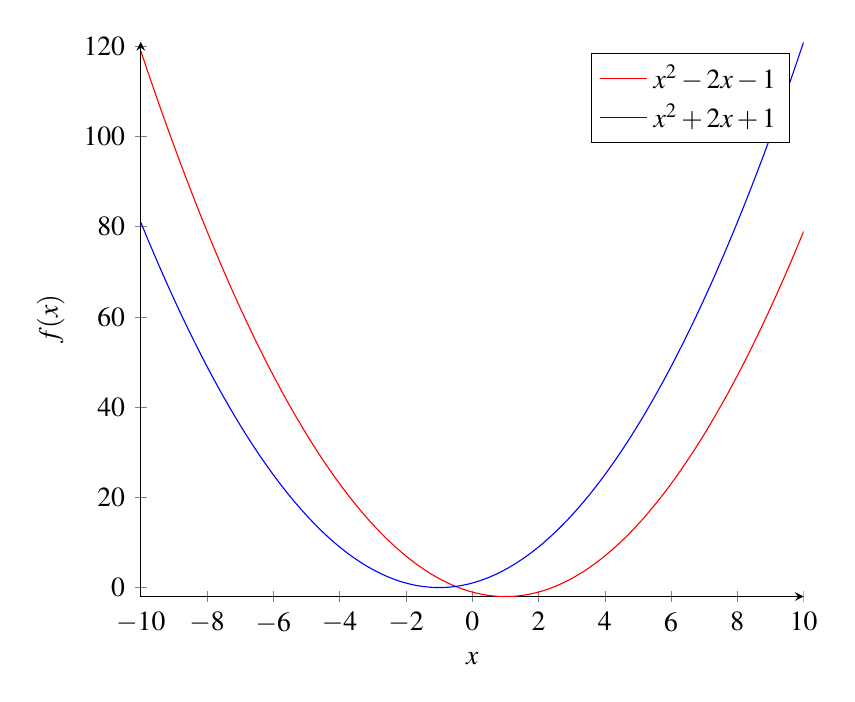
\begin{tikzpicture}
\begin{axis}[
    axis lines = left,
    xlabel = $x$,
    ylabel = {$f(x)$},
]
%Below the red parabola is defined
\addplot [
    domain=-10:10, 
    samples=100, 
    color=red,
]
{x^2 - 2*x - 1};
\addlegendentry{$x^2 - 2x - 1$}
%Here the blue parabloa is defined
\addplot [
    domain=-10:10, 
    samples=100, 
    color=blue,
    ]
    {x^2 + 2*x + 1};
\addlegendentry{$x^2 + 2x + 1$}
 
\end{axis}
\end{tikzpicture}


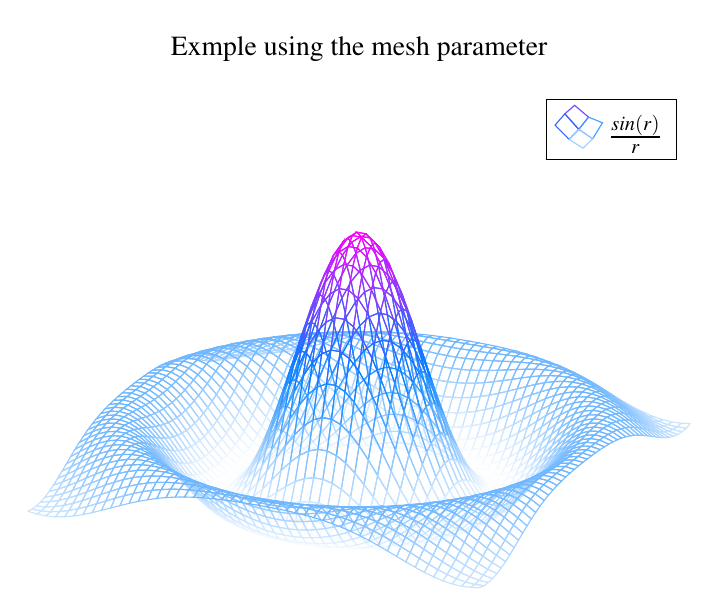
\begin{tikzpicture}
\begin{axis}[
    title=Exmple using the mesh parameter,
    hide axis,
    colormap/cool,
]
\addplot3[
    mesh,
    samples=50,
    domain=-8:8,
]
{sin(deg(sqrt(x^2+y^2)))/sqrt(x^2+y^2)};
\addlegendentry{$\frac{sin(r)}{r}$}
\end{axis}
\end{tikzpicture}

\begin{figure}[h]
    \centering 
   \includegraphics[scale=0.3]{wormhole0.jpg}
    \label{fig:wormhole}
\end{figure}


        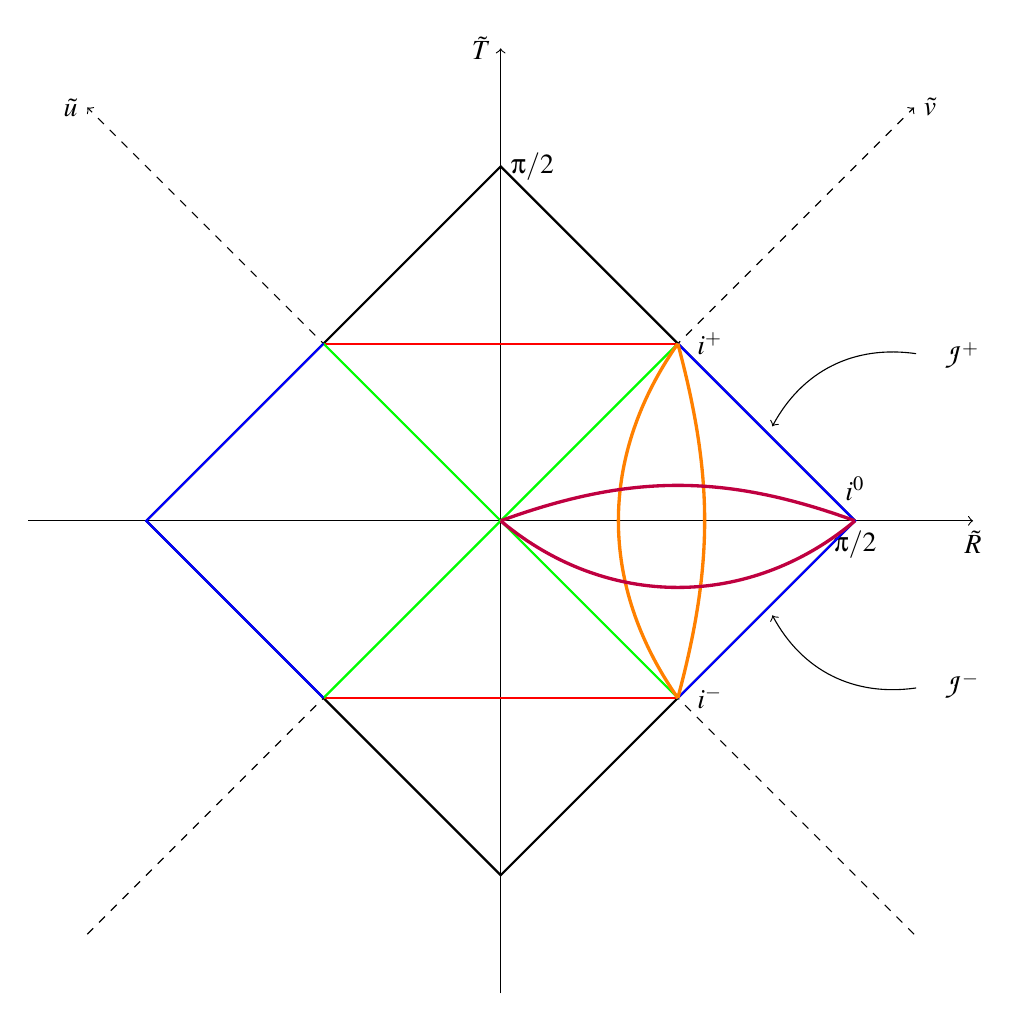
\begin{tikzpicture}[scale=1.5]
            \draw[->] (-4,0) -- (4,0) node[below] {$\tilde{R}$};
            \draw[->] (0,-4) -- (0,4) node[left] {$\tilde{T}$};
            \draw[dashed,->] (-3.5,-3.5) -- (3.5,3.5) node[right] {$\tilde{v}$};
            \draw[dashed,->] (3.5,-3.5) -- (-3.5,3.5) node[left] {$\tilde{u}$};
            \draw[thick] (3,0) node[below] {$\pi/2$} -- (0,3) node[right] {$\pi/2$} -- (-3,0) -- (0,-3) -- cycle;
            \draw[red,thick] (-1.5,1.5) -- (1.5,1.5);
            \draw[red,thick] (-1.5,-1.5) -- (1.5,-1.5);
            \draw[green,thick] (-1.5,-1.5) -- (1.5,1.5);
            \draw[green,thick] (-1.5,1.5) -- (1.5,-1.5);
            \draw[blue,thick] (1.5,-1.5) -- (3,0) -- (1.5,1.5);
            \draw[blue,thick] (-1.5,-1.5) -- (-3,0) -- (-1.5,1.5);
            \draw[orange,bend left=15,very thick] (1.5,1.5) to (1.5,-1.5);
            \draw[orange,bend right=35,very thick] (1.5,1.5) to (1.5,-1.5);
            \draw[purple,bend left=20,very thick] (0,0) to (3,0);
            \draw[purple,bend right=40,very thick] (0,0) to (3,0);
            \node[label=right:$i^+$] (1) at (1.5,1.5) {};
            \node[label=right:$i^-$] (2) at (1.5,-1.5) {};
            \node[label=above:$i^0$] (3) at (3,0) {};

            
            \node[label=right:$\mathcal{J}^+$] (4) at (3.6,1.4) {};
            \node[label=right:$\mathcal{J}^-$] (5) at (3.6,-1.4) {};

            \draw[->,bend right=35] (4) to (2.3,0.8);
            \draw[->,bend left=35] (5) to (2.3,-0.8);
        \end{tikzpicture}







\begin{thebibliography}{22} 



\bibitem{ligo} Berti, E. (2016). The First Sounds of Merging Black Holes. \textit{APS Physics}, 9, 17. doi:10.1103/Physics.9.17

\end{thebibliography}

\end{document}
